\documentclass[compress,trans,9pt]{beamer}
% \documentclass[9pt]{beamer}
%\documentclass[compress,9pt,usenames,dvipsnames]{beamer}
% \usepackage[utf8]{inputenc}
% \includeonlyframes{current}
\setbeamercovered{dynamic}
\usepackage{etex}
\usepackage{graphicx,url,psfrag}
\usepackage{tikz}
\usetikzlibrary{
  decorations.pathreplacing,
  calc,
  decorations.fractals,
  through,
  shapes,
  patterns,
  arrows.meta,
  decorations.pathreplacing,
  arrows,
  shapes,
  mindmap
}
\usepackage[center]{subfigure}
\usepackage{enumerate}
\usepackage[makeroom]{cancel}
\usepackage{mathtools}
\usepackage{graphbox}
\usepackage{amssymb}
% \usepackage[showframe]{geometry}
% \usepackage{enumitem}

%
% for warning sign
%
\usepackage{stackengine}
\usepackage{scalerel}
\usepackage{xcolor}
\newcommand\dangersign[1][2ex]{%
  \renewcommand\stacktype{L}%
  \scaleto{\stackon[1.3pt]{\color{red}$\triangle$}{\tiny !}}{#1}%
}
% %  The following is to show codes:
\usepackage{listings}
% \usepackage{color}
\usepackage{colortbl}
\usepackage{dbt}

\definecolor{dkgreen}{rgb}{0,0.6,0}
\definecolor{gray}{rgb}{0.5,0.5,0.5}
\definecolor{mauve}{rgb}{0.58,0,0.82}

% \definecolor{deepblue}{rgb}{0,0,0.5}
% \definecolor{deepred}{rgb}{0.6,0,0}
% \definecolor{deepgreen}{rgb}{0,0.5,0}
% \lstset{
%   language=Python,
%   backgroundcolor=\color{red},  % choose the background color. You must add \usepackage{color}
%   % backgroundcolor=\color{background},  % choose the background color. You must add \usepackage{color}
%   basicstyle=\footnotesize,
%   otherkeywords={self},
%   keywordstyle=\ttb\color{deepblue},
%   emph={MyClass,__init__},
%   emphstyle=\ttb\color{deepred},
%   stringstyle=\color{deepgreen},
%   commentstyle=\color{red},  %%%%%%%%
%   frame=tb,
%   showstringspaces=false
% }
%
% \lstdefinestyle{Python}{
%     language        = Python,
%     basicstyle      = \footnotesize,
%     keywordstyle    = \color{blue},
%     keywordstyle    = [2] \color{red}, % just to check that it works
%     stringstyle     = \color{green},
%     commentstyle    = \color{red}\ttfamily
% }

\lstset{frame=tb,
  language=Java,
  aboveskip=3mm,
  belowskip=3mm,
  showstringspaces=false,
  columns=flexible,
  basicstyle={\small\ttfamily},
  numbers=none,
  numberstyle=\tiny\color{gray},
  keywordstyle=\color{blue},
  commentstyle=\color{dkgreen},
  stringstyle=\color{mauve},
  breaklines=true,
  breakatwhitespace=true,
  tabsize=3
}
\lstset{language=Java}

\lstset{ %
  language=R,                     % the language of the code
  basicstyle=\footnotesize,       % the size of the fonts that are used for the code
  numbers=left,                   % where to put the line-numbers
  numberstyle=\tiny\color{gray},  % the style that is used for the line-numbers
  stepnumber=1,                   % the step between two line-numbers. If it's 1, each line
                                  % will be numbered
  numbersep=5pt,                  % how far the line-numbers are from the code
  backgroundcolor=\color{background},  % choose the background color. You must add \usepackage{color}
  showspaces=false,               % show spaces adding particular underscores
  showstringspaces=false,         % underline spaces within strings
  showtabs=false,                 % show tabs within strings adding particular underscores
  frame=single,                   % adds a frame around the code
  rulecolor=\color{black},        % if not set, the frame-color may be changed on line-breaks within not-black text (e.g. commens (green here))
  tabsize=2,                      % sets default tabsize to 2 spaces
  captionpos=b,                   % sets the caption-position to bottom
  breaklines=true,                % sets automatic line breaking
  breakatwhitespace=false,        % sets if automatic breaks should only happen at whitespace
  title=\lstname,                 % show the filename of files included with \lstinputlisting;
                                  % also try caption instead of title
  keywordstyle=\color{blue},      % keyword style
  commentstyle=\color{dkgreen},   % comment style
  stringstyle=\color{mauve},      % string literal style
  escapeinside={\%*}{*)},         % if you want to add a comment within your code
  morekeywords={*,...}            % if you want to add more keywords to the set
}
% \usepackage[usenames,dvipsnames]{color}
% \lstset{
%   language=Python,                     % the language of the code
%   basicstyle=\footnotesize,       % the size of the fonts that are used for the code
%   numbers=left,                   % where to put the line-numbers
%   numberstyle=\tiny\color{gray},  % the style that is used for the line-numbers
%   stepnumber=1,                   % the step between two line-numbers. If it's 1, each line
%                                   % will be numbered
%   numbersep=5pt,                  % how far the line-numbers are from the code
%   backgroundcolor=\color{background},  % choose the background color. You must add \usepackage{color}
%   showspaces=false,               % show spaces adding particular underscores
%   showstringspaces=false,         % underline spaces within strings
%   showtabs=false,                 % show tabs within strings adding particular underscores
%   frame=single,                   % adds a frame around the code
%   rulecolor=\color{black},        % if not set, the frame-color may be changed on line-breaks within not-black text (e.g. commens (green here))
%   tabsize=2,                      % sets default tabsize to 2 spaces
%   captionpos=b,                   % sets the caption-position to bottom
%   breaklines=true,                % sets automatic line breaking
%   breakatwhitespace=false,        % sets if automatic breaks should only happen at whitespace
%   title=\lstname,                 % show the filename of files included with \lstinputlisting;
%                                   % also try caption instead of title
%   keywordstyle=\ttb\color{blue},      % keyword style
%   commentstyle=\color{dkgreen},   % comment style
%   stringstyle=\color{mauve},      % string literal style
%   escapeinside={\%*}{*)},         % if you want to add a comment within your code
%   morekeywords={*,...}            % if you want to add more keywords to the set
% }

% \usepackage[dvipsnames]{xcolor}
% \newcommand{\Cross}{\mathbin{\tikz [x=1.4ex,y=1.4ex,line width=.2ex] \draw (0,0) -- (1,1) (0,1) -- (1,0);}}%
\newcommand{\Crossme}[1]{\!\!
\tikz [black,x=1.1em,y=1.1em,line width=.4ex]
\draw (-0.5,-0.5) -- (0,0) node {\footnotesize #1} -- (0.5,0.5) (0.5,-0.5) -- (-0.5,0.5);}%
\newcommand{\Checkme}[1]{\!\!
\tikz [x=1.1em,y=1.1em,line width=.4ex]
\draw [black] (0,0.7) -- (0.3,0) --(0.9,1.0) (0.5,0.5) node {\footnotesize #1};}
% \beamerdefaultoverlayspecification{<+-| alert@+>} %(this will show line by line)
\beamerdefaultoverlayspecification{<+->} %(this will show line by

% \usepackage{natbib}
% \input{../myMathSymbols.tex}
% \newcommand{\tlMr}[4]{\:{}^{\hspace{0.2em}#1}_{#2} \hspace{-0.1em}#3_{#4}}

% Smiley face\Smiley{} \Frowny{}
\usepackage{marvosym}
% -------------------------------------------------
%  Set directory for figs
% -------------------------------------------------
\usepackage{grffile}
\graphicspath{{Codes/}}
% -------------------------------------------------
%  Define colors
% -------------------------------------------------
\def\refcolor{cyan}
\newcommand{\myref}[1]{\small {\em #1}}
\def\excolor{brown}
% \usepackage{color}
% \usepackage[dvipsnames]{xcolor}


% % % Define danger sign
\newcommand*{\TakeFourierOrnament}[1]{{%
\fontencoding{U}\fontfamily{futs}\selectfont\char#1}}
\newcommand*{\danger}{\TakeFourierOrnament{66}}


% -------------------------------------------------
%  Define short-hand symbols.
% -------------------------------------------------
\newcommand{\B}{\textbf{B}}
\newcommand{\PP}{\mathbb{P}}
\newcommand{\E}{\mathbb{E}}
\newcommand{\D}{\mathbb{D}}
\newcommand{\W}{\dot{W}}
\newcommand{\ud}{\ensuremath{\mathrm{d}}}
\newcommand{\Ceil}[1]{\left\lceil #1 \right\rceil}
\newcommand{\Floor}[1]{\left\lfloor #1 \right\rfloor}
\newcommand{\sgn}{\text{sgn}}
\newcommand{\Lad}{\text{L}_{\text{ad}}^2}
\newcommand{\SI}[1]{\mathcal{I}\left[#1 \right]}
\newcommand{\SIB}[2]{\mathcal{I}_{#2}\left[#1 \right]}
\newcommand{\Indt}[1]{1_{\left\{#1 \right\}}}
\newcommand{\LadInPrd}[1]{\left\langle #1 \right\rangle_{\text{L}_\text{ad}^2}}
\newcommand{\LadNorm}[1]{\left|\left|  #1 \right|\right|_{\text{L}_\text{ad}^2}}
\newcommand{\Norm}[1]{\left|\left|  #1   \right|\right|}
\newcommand{\Ito}{It\^{o} }
\newcommand{\Itos}{It\^{o}'s }
\newcommand{\spt}[1]{\text{supp}\left(#1\right)}
\newcommand{\InPrd}[1]{\left\langle #1 \right\rangle}
\newcommand{\mr}{\textbf{r}}
\newcommand{\Ei}{\text{Ei}}
\newcommand{\arctanh}{\operatorname{arctanh}}
\newcommand{\ind}[1]{\mathbb{I}_{\left\{ {#1} \right\} }}
\newcommand{\Var}{\text{Var}}
\newcommand{\Cov}{\text{Cov}}
\newcommand{\Corr}{\text{Corr}}

\newcommand{\baseurl}[1]{\footnotesize\url{http://math.emory.edu/~lchen41/teaching/2020_Spring/#1}}


\newcommand*\mystrut[1]{\vrule width0pt height0pt depth#1\relax} % adding vertical space

\DeclareMathOperator{\esssup}{\ensuremath{ess\,sup}}

\newcommand{\steps}[1]{\vskip 0.3cm \textbf{#1}}
\newcommand{\calB}{\mathcal{B}}
\newcommand{\calC}{\mathcal{C}}
\newcommand{\calD}{\mathcal{D}}
\newcommand{\calE}{\mathcal{E}}
\newcommand{\calF}{\mathcal{F}}
\newcommand{\calG}{\mathcal{G}}
\newcommand{\calK}{\mathcal{K}}
\newcommand{\calH}{\mathcal{H}}
\newcommand{\calI}{\mathcal{I}}
\newcommand{\calL}{\mathcal{L}}
\newcommand{\calM}{\mathcal{M}}
\newcommand{\calN}{\mathcal{N}}
\newcommand{\calO}{\mathcal{O}}
\newcommand{\calT}{\mathcal{T}}
\newcommand{\calP}{\mathcal{P}}
\newcommand{\calR}{\mathcal{R}}
\newcommand{\calS}{\mathcal{S}}
\newcommand{\calV}{\mathcal{V}}
\newcommand{\bbC}{\mathbb{C}}
\newcommand{\bbN}{\mathbb{N}}
\newcommand{\bbP}{\mathbb{P}}
\newcommand{\bbZ}{\mathbb{Z}}
\newcommand{\myVec}[1]{\overrightarrow{#1}}
\newcommand{\sincos}{\begin{array}{c} \cos \\ \sin \end{array}\!\!}
\newcommand{\CvBc}[1]{\left\{\:#1\:\right\}}
\newcommand*{\one}{{{\rm 1\mkern-1.5mu}\!{\rm I}}}

\newcommand{\OneFrame}[1]{
\begin{enumerate}\item[#1] \phantom{av} \\[20em]\vfill\phantom{av}\myEnd\end{enumerate}}

\newcommand{\bH}{\ensuremath{\mathrm{H}}}
\newcommand{\Ai}{\ensuremath{\mathrm{Ai}}}

\newcommand{\R}{\mathbb{R}}
\newcommand{\myEnd}{\hfill$\square$}
\newcommand{\myQED}{\hfill\textcolor{lgtblue}{$\blacksquare$}}
\newcommand{\ds}{\displaystyle}
\newcommand{\Shi}{\text{Shi}}
\newcommand{\Chi}{\text{Chi}}
\newcommand{\Erf}{\ensuremath{\mathrm{erf}}}
\newcommand{\Erfc}{\ensuremath{\mathrm{erfc}}}
\newcommand{\He}{\ensuremath{\mathrm{He}}}
\newcommand{\Res}{\ensuremath{\mathrm{Res}}}

\newcommand{\mySeparateLine}{\begin{center}
 \makebox[\linewidth]{\rule{0.6\paperwidth}{0.4pt}}
\end{center}}

\theoremstyle{definition}
% \newtheorem{definition}[theorem]{Definition}
% \newtheorem{hypothesis}[theorem]{Hypothesis}
\newtheorem{assumption}[theorem]{Assumption}

\theoremstyle{plain}
% \newtheorem{theorem}{Theorem}
% \newtheorem{corollary}[theorem]{Corollary}
% \newtheorem{lemma}[theorem]{Lemma}
\newtheorem{proposition}[theorem]{Proposition}

\mode<presentation>
{
%      \usetheme{Warsaw}
%     \usetheme{JuanLesPins}
%  \usetheme{Hannover}
%  \usetheme{Montpellier}
   \useoutertheme{default}
  % or ...

  \setbeamercovered{transparent}
  % or whatever (possibly just delete it)
 \setbeamertemplate{frametitle}{
  \begin{centering}
    \color{blue}
    {\insertframetitle}
    \par
  \end{centering}
  }
}
\usefoottemplate{\hfill \insertframenumber{}}
% \inserttotalframenumber

\usepackage[english]{babel}
% or whatever

% \usepackage[latin1]{inputenc}
% or whatever

\usepackage{times}
\usepackage[T1]{fontenc}
% Or whatever. Note that the encoding and the font should match. If T1
% does not look nice, try deleting the line with the fontenc.

% \DeclareMathOperator{\Lip}{Lip}
\DeclareMathOperator{\lip}{l}
% \DeclareMathOperator{\Vip}{\overline{v}}
% \DeclareMathOperator{\vip}{\underline{v}}
% \DeclareMathOperator{\vv}{v}
% \DeclareMathOperator{\BC}{BC}
% \DeclareMathOperator{\CH}{CD}

\usepackage{pgfpages}
% \setbeameroption{show notes}
% \setbeamertemplate{note page}[plain]
% \setbeameroption{second mode text on second screen=right}
% \setbeameroption{show notes on second screen=right}
%
\title % (optional, use only with long paper titles)
{
Math 362: Mathematical Statistics II
}

% \subtitle
% {Research Plan} % (optional)

\author{Le Chen\\
\url{le.chen@emory.edu}\\
\url{chenle02@gmail.com}\\[2em]
Emory University\\
Atlanta, GA\\[2em]
\textcolor{gray}{\small Last updated on Spring 2021}\\
\textcolor{gray}{\small Last compiled on \today}
}
\institute[Emory University]
{%
\vspace{3em}
% \pgfuseimage{UNLV}
 }
 \vfill
% - Use the \inst command only if there are several affiliations.
% - Keep it simple, no one is interested in your street address.

% \date[Talk at Karlsruhe] % (optional)
% {\today }
 \date[Columbus]{
   2021 Spring\\[1em]
   Creative Commons License\\
   (CC By-NC-SA)
 }

\subject{}
% This is only inserted into the PDF information catalog. Can be left
% out.

% If you have a file called "university-logo-filename.xxx", where xxx
% is a graphic format that can be processed by latex or pdflatex,
% resp., then you can add a logo as follows:

% \pgfdeclareimage[height=0.8cm]{UNLV}{figs/UNLV-186.png}

% Delete this, if you do not want the table of contents to pop up at
% the beginning of each subsection:
% \AtBeginSubsection[]
% {
%   \begin{frame}<beamer>{Outline}
%     \tableofcontents[currentsection,currentsubsection]
%   \end{frame}
% }


% If you wish to uncover everything in a step-wise fashion, uncomment
% the following command:

% \beamerdefaultoverlayspecification{<+->}
% % % % % % % % % % % % % % % % % % %
%  Define a block
% % % % % % % % % % % % % % % % % % %
\newenvironment<>{problock}[1]{%
  \begin{actionenv}#2%
      \def\insertblocktitle{#1}%
      \par%
      \mode<presentation>{%
        \setbeamercolor{block title}{fg=white,bg=olive!95!black}
       \setbeamercolor{block body}{fg=black,bg=olive!25!white}
       \setbeamercolor{itemize item}{fg=white!20!white}
       \setbeamertemplate{itemize item}[triangle]
     }%
      \usebeamertemplate{block begin}}
    {\par\usebeamertemplate{block end}\end{actionenv}}

\newenvironment<>{assblock}[1]{%
  \begin{actionenv}#2%
      \def\insertblocktitle{#1}%
      \par%
      \mode<presentation>{%
        \setbeamercolor{block title}{fg=white,bg=green!50!black}
       \setbeamercolor{block body}{fg=black,bg=green!10}
       \setbeamercolor{itemize item}{fg=green!80!black}
       \setbeamertemplate{itemize item}[triangle]
     }%
      \usebeamertemplate{block begin}}
    {\par\usebeamertemplate{block end}\end{actionenv}}


\newcommand{\mySection}[1]{\section{\S\: #1}\begin{frame}{\myChapter}\tableofcontents[currentsection]\end{frame}}

\AtBeginSection[]
  {
     \begin{frame}<beamer>
     \frametitle{Plan}
     \tableofcontents[currentsection]
     \end{frame}
  }


\begin{document}

\AtBeginSection[]
  {
     \begin{frame}<beamer>
     \frametitle{Plan}
     \tableofcontents[currentsection]
     \end{frame}
  }


%-------------- start slide -------------------------------%{{{
\begin{frame}[noframenumbering]
  \titlepage
\end{frame}
%-------------- end slide -------------------------------%}}}


% \begin{frame}{Outline}
%   \tableofcontents
%   % You might wish to add the option [pausesections]
% \end{frame}


\newcommand{\myChapter}{Chapter 13. Randomized Block Designs}

%-------------- start slide -------------------------------%{{{
\begin{frame}
\begin{center}
\huge
\myChapter
\end{center}
\end{frame}
%-------------- end slide -------------------------------%}}}

\mySection{13.1 Introduction}
%-------------- start slide -------------------------------%{{{ 13.4
\begin{frame}
	% {\S\: 13.1 Introduction}
	\begin{center}
		{\bf Rationale:}\\[1em]Reducing variability by blocking$^\dagger$
		\vfill
		{\small {\it $^\dagger$ Blocking} is the arranging of experimental units in groups (blocks) that are similar to one another.}
		\vfill
		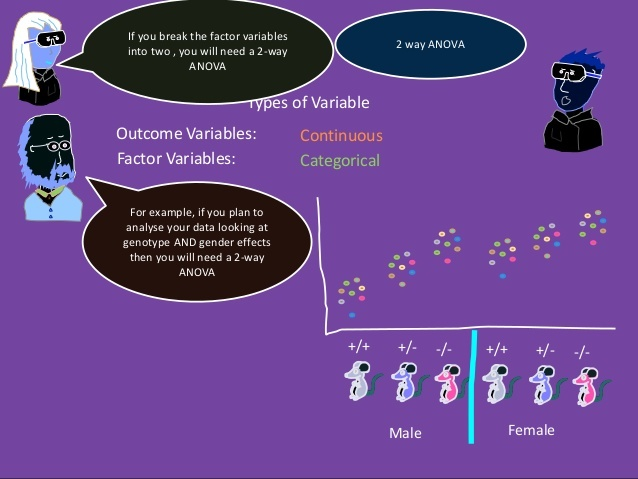
\includegraphics[scale=0.25]{experimental-design-cartoon-neg.jpg}
		\vfill
		{\footnotesize
		\url{https://www.slideshare.net/KevinHamill2/experimental-design-cartoon-part-5-sample-size}}
	\end{center}
\end{frame}
%-------------- end slide -------------------------------%}}}
%-------------- start slide -------------------------------%{{{ 13.5
\begin{frame}[fragile]
	\centering
	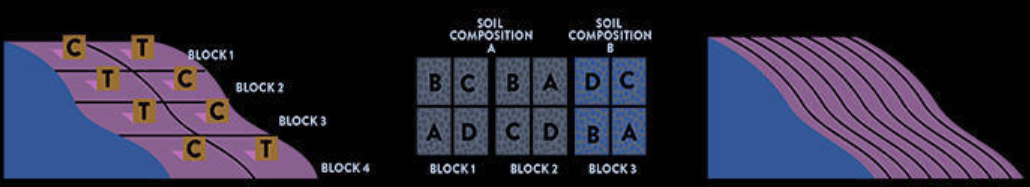
\includegraphics[scale=0.3]{Addressing-Field.png}
	\vfill

	\begin{minipage}{0.6\textwidth}
	\begin{enumerate}
	\item[Goal] Reducing variability caused by
	\item[a]  {\it elevation}.
	\item[b]  {\it soil types}.
	\item[]  \qquad {v.s.}
	\item[c] {\it complete randomized design}
	\end{enumerate}
	\end{minipage}
\hfill\pause
	\begin{minipage}{0.35\textwidth}
		\vspace{1.8em}
	\begin{enumerate}
	\item[]
		$\scalebox{2.2}{\}}$\hfill One-way ANOVA
		% \[
		% \scalebox{2.2}{\}}\:\text{One-way ANOVA}
		% \]
		\vspace{1.4em}
	\item[]\hfill Two-way ANOVA
	\end{enumerate}
	\end{minipage}

	\vfill
	{\footnotesize\url{https://www.sare.org/Learning-Center/Bulletins/How-to-Conduct-Research-on-Your-Farm-or-Ranch/Text-Version/Basics-of-Experimental-Design}}
\end{frame}
%-------------- end slide -------------------------------%}}}

\mySection{13.2 The $F$ Test for a Randomized Block Design}
%-------------- start slide -------------------------------%{{{
\begin{frame}
	% {\S\: 13.2 The $F$ Test for a Randomized Block Design}

	\begin{enumerate}
		\item[Setup] $Y_{ij}$ indep. $\sim N(\mu_j+\beta_i,\sigma^2)$, i.e., $Y_{ij} = \mu_j+\beta_i+\epsilon_{ij}$, $\epsilon_{ij}$ i.i.d. $\sim N(0,\sigma^2)$
			\vfill
		\item[]
			\begin{center}
				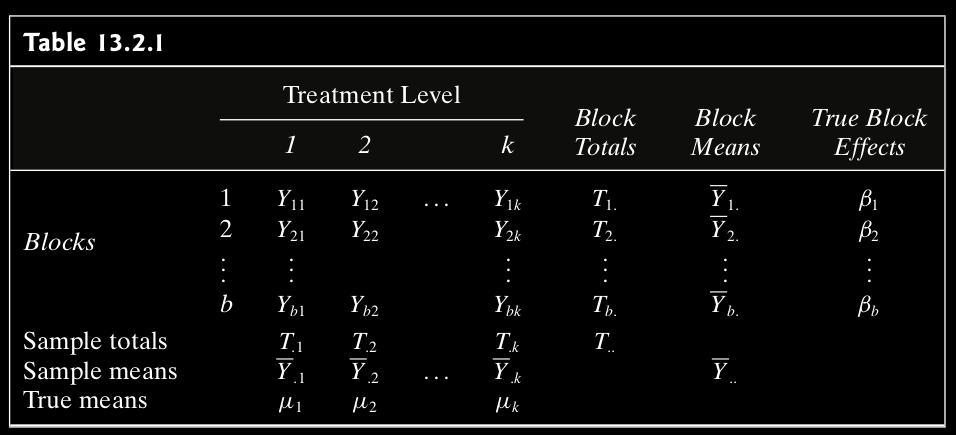
\includegraphics[scale=0.25]{Table_13-2-1-neg.png}
			\end{center}
	\end{enumerate}
\end{frame}
%-------------- end slide -------------------------------%}}}
%-------------- start slide -------------------------------%{{{
\begin{frame}[fragile]
	\begin{enumerate}
		\item[Recall] For one-way ANOVA,
			\[
				Y_{ij} = \textcolor{red}{\mu_j} + \epsilon_{ij}
			\]
		\item[]
			\[\Downarrow\]
		\item[]
	\begin{align*}
		SSTOT = & \sum_{i=1}^b\sum_{j=1}^k \left(Y_{ij}-\overline{Y}_{\cdot\cdot} \right)^2
		     \\ & =  \sum_{i=1}^b\sum_{j=1}^k\left[ \left(Y_{ij}-\textcolor{red}{\overline{Y}_{\cdot j}} \right)+\left(\textcolor{red}{\overline{Y}_{\cdot j}} - \overline{Y}_{\cdot\cdot}\right)\right]^2
		     \\ & =  \sum_{i=1}^b\sum_{j=1}^k\left(Y_{ij}-\overline{Y}_{\cdot j} \right)^2+ \text{zero cross term}+\sum_{i=1}^b\sum_{j=1}^k\left(\overline{Y}_{\cdot j} - \overline{Y}_{\cdot\cdot}\right)^2
		     \\ & =  \sum_{i=1}^b\sum_{j=1}^k\left(Y_{ij}-\overline{Y}_{\cdot j} \right)^2+ \textcolor{red}{b\sum_{j=1}^k \left(\overline{Y}_{\cdot j} - \overline{Y}_{\cdot\cdot}\right)^2
}		      \\&= SSE +\textcolor{red}{SSTR}
	\end{align*}
	\end{enumerate}
\end{frame}
%-------------- end slide -------------------------------%}}}
%-------------- start slide -------------------------------%{{{
\begin{frame}[fragile]
	\begin{center}
		\begin{tabular}{ccccc}
			$\displaystyle SSTOT$ &
			= &
			$\displaystyle SSE$ &
			+ &
			$\displaystyle \textcolor{red}{SSTR}$ \\ \\
			  &$\Downarrow$&&& \\ \\
			$\displaystyle \frac{SSTOT}{\sigma^2}$ &
			= &
			$\displaystyle \frac{SSE}{\sigma^2}$ &
			+ &
			$\displaystyle \frac{\textcolor{red}{SSTR}}{\sigma^2}$ \\ \\
			$\wr$&& $\wr$ &  & $\wr$ \\ \\
			$\chi^2(bk-1)$ && $\chi^2(bk-k)$ & $\perp$ & $\chi^2(k-1)$
			\\[2em]
			Under $H_0$& & \checkmark && Under $H_0$
		\end{tabular}
\vfill
\[
H_0: \mu_1=\cdots =\mu_k
\]
	\end{center}
\end{frame}
%-------------- end slide -------------------------------%}}}
%-------------- start slide -------------------------------%{{{
\begin{frame}[fragile]
	\begin{enumerate}
		\item[Symmetry] If
			\[
				Y_{ij} = \textcolor{cyan}{\beta_i} + \epsilon_{ij}
			\]
		\item[]
			\[\Downarrow\]
		\item[]
	\begin{align*}
		SSTOT = & \sum_{i=1}^b\sum_{j=1}^k \left(Y_{ij}-\overline{Y}_{\cdot\cdot} \right)^2
		     \\ & =  \sum_{i=1}^b\sum_{j=1}^k\left[ \left(Y_{ij}-\textcolor{cyan}{\overline{Y}_{i\cdot}} \right)+\left(\textcolor{cyan}{\overline{Y}_{i\cdot}} - \overline{Y}_{\cdot\cdot}\right)\right]^2
		     \\ & =  \sum_{i=1}^b\sum_{j=1}^k\left(Y_{ij}-\overline{Y}_{i\cdot} \right)^2+ \text{zero cross term}+\sum_{i=1}^b\sum_{j=1}^k\left(\overline{Y}_{i\cdot} - \overline{Y}_{\cdot\cdot}\right)^2
		     \\ & =  \sum_{i=1}^b\sum_{j=1}^k\left(Y_{ij}-\overline{Y}_{i\cdot} \right)^2+ \textcolor{cyan}{k\sum_{i=1}^b\left(\overline{Y}_{i\cdot} - \overline{Y}_{\cdot\cdot}\right)^2
}		      \\&= SSE +\textcolor{cyan}{SSB}
	\end{align*}
	\end{enumerate}
\end{frame}
%-------------- end slide -------------------------------%}}}
%-------------- start slide -------------------------------%{{{
\begin{frame}[fragile]
	\begin{center}
		\begin{tabular}{ccccc}
			$\displaystyle SSTOT$ &
			= &
			$\displaystyle SSE$ &
			+ &
			$\displaystyle \textcolor{cyan}{SSB}$ \\ \\
			  &$\Downarrow$&&& \\ \\
			$\displaystyle \frac{SSTOT}{\sigma^2}$ &
			= &
			$\displaystyle \frac{SSE}{\sigma^2}$ &
			+ &
			$\displaystyle \frac{\textcolor{cyan}{SSB}}{\sigma^2}$ \\ \\
			$\wr$&& $\wr$ &  & $\wr$ \\ \\
			$\chi^2(bk-1)$ && $\chi^2(bk-b)$ & $\perp$ & $\chi^2(b-1)$
			\\[2em]
			Under $\widetilde H_0$& & \checkmark && Under $\widetilde H_0$
		\end{tabular}
		\vfill
		\[
		\widetilde H_0 : \beta_1=\cdots = \beta_b
		\]
	\end{center}
\end{frame}
%-------------- end slide -------------------------------%}}}
%-------------- start slide -------------------------------%{{{
\begin{frame}[fragile]
	\begin{enumerate}
		\item[Similarly] If
			\[
				Y_{ij} = \textcolor{red}{\mu_j} + \textcolor{cyan}{\beta_i} + \epsilon_{ij}
			\]
		\item[]
			\[\Downarrow\]
		\item[]
	\begin{align*}
		\hspace{-4em}SSTOT =  & \sum_{i=1}^b\sum_{j=1}^k \left(Y_{ij}-\overline{Y}_{\cdot\cdot} \right)^2 \\
                          & =  \sum_{i=1}^b\sum_{j=1}^k\left[ \left(Y_{ij}-\textcolor{cyan}{\overline{Y}_{i\cdot}} - \textcolor{red}{\overline{Y}_{\cdot j}}+\overline{Y}_{\cdot\cdot} \right)+\left(\textcolor{cyan}{\overline{Y}_{i\cdot}} - \overline{Y}_{\cdot\cdot}\right)+\left(\textcolor{red}{\overline{Y}_{\cdot j}}- \overline{Y}_{\cdot\cdot}\right)\right]^2 \\
													& =  \sum_{i=1}^b\sum_{j=1}^k\left(Y_{ij}-\overline{Y}_{i\cdot} -\overline{Y}_{\cdot j}+\overline{Y}_{\cdot\cdot}\right)^2 +\sum_{i=1}^b\sum_{j=1}^k\left(\overline{Y}_{i\cdot} - \overline{Y}_{\cdot\cdot}\right)^2 \\
													&\quad+\sum_{i=1}^b\sum_{j=1}^k\left(\overline{Y}_{\cdot j} - \overline{Y}_{\cdot\cdot}\right)^2 + \text{zero cross terms} \\
													& =  \sum_{i=1}^b\sum_{j=1}^k\left(Y_{ij}-\overline{Y}_{i\cdot} -\overline{Y}_{\cdot j} + \overline{Y}_{\cdot\cdot} \right)^2+\textcolor{cyan}{k\sum_{i=1}^b\left(\overline{Y}_{i\cdot} - \overline{Y}_{\cdot\cdot}\right)^2} +\textcolor{red}{b\sum_{j=1}^k\left(\overline{Y}_{\cdot j} - \overline{Y}_{\cdot\cdot}\right)^2} \\
													&= SSE + \textcolor{cyan}{SSB} + \textcolor{red}{SSTR}
	\end{align*}
	\end{enumerate}
\end{frame}
%-------------- end slide -------------------------------%}}}
%-------------- start slide -------------------------------%{{{
\begin{frame}[fragile]
	\begin{center}
		\begin{tabular}{ccccccc}
			$\displaystyle SSTOT$ &
			= &
			$\displaystyle SSE$ &
			+ &
			$\displaystyle \textcolor{cyan}{SSB}$ &+& $\displaystyle \textcolor{red}{SSTR}$ \\ \\
					    &$\Downarrow$&&& &&\\ \\
			$\displaystyle \frac{SSTOT}{\sigma^2}$ &
			= &
			$\displaystyle \frac{SSE}{\sigma^2}$ &
			+ &
			$\displaystyle \frac{\textcolor{cyan}{SSB}}{\sigma^2}$ &+& $\displaystyle \frac{\textcolor{red}{SSTR}}{\sigma^2}$ \\ \\
			$\wr$&& $\wr$ &  & $\wr$ && $\wr$ \\ \\
			$\chi^2(bk-1)$ && $\chi^2((k-1)(b-1))$ & $\perp$ & $\chi^2(b-1)$ & $\perp$ & $\chi^2(k-1)$
			\\[2em]
			Under $H_0$ or $\widetilde H_0$& &\checkmark&& under $\widetilde{H}_0$ && under $H_0$
		\end{tabular}
		\vfill
		\[
		\widetilde H_0 : \beta_1=\cdots = \beta_b
		\qquad\text{and}\qquad
		H_0: \mu_1\cdots = \mu_k
		\]
	\end{center}
\end{frame}
%-------------- end slide -------------------------------%}}}
%-------------- start slide -------------------------------%{{{
\begin{frame}[fragile]


	\phantom{a}\hfill\begin{minipage}{0.6\textwidth}
		\[
		H_0: \mu_1\cdots = \mu_k
		\]
		\[
		\Downarrow
		\]
	\end{minipage}

% \vfill
	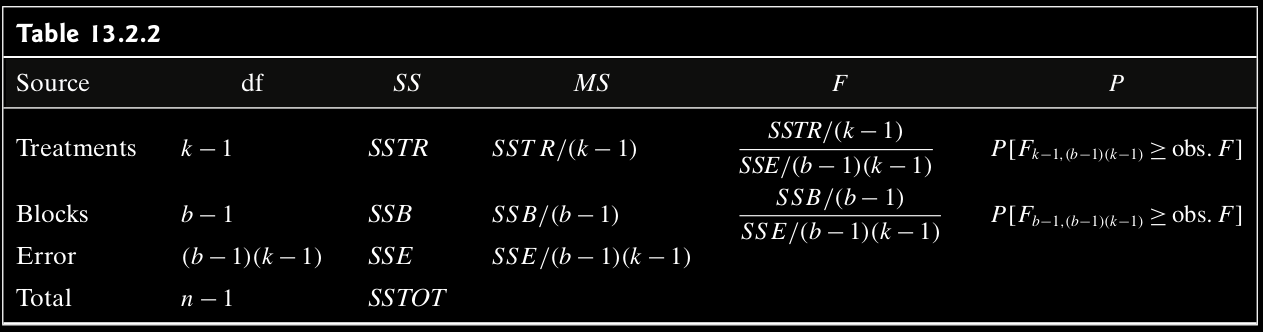
\includegraphics[scale=0.25]{Table_13-2-2-neg.png}
% \vfill

	\phantom{a}\hfill\begin{minipage}{0.6\textwidth}
		\[
		\Uparrow
		\]
	\[
		\widetilde H_0 : \beta_1=\cdots = \beta_b
	\]
	\end{minipage}
\end{frame}
%-------------- end slide -------------------------------%}}}
%-------------- start slide -------------------------------%{{{
\begin{frame}[fragile]{Computing formulas}
\[
	C =  \frac{T_{\cdot\cdot}^2}{bk}
\]
\vfill
\[
	\textcolor{red}{SSTR} = b\sum_{j=1}^k\left(\overline{Y}_{\cdot j}-\overline{Y}_{\cdot\cdot}\right)^2
	= b\sum_{j=1}^k \overline{Y}_{\cdot j}^2 - bk \overline{Y}_{\cdot\cdot}^2 =
	\frac{1}{b}\sum_{j=1}^k \overline{T}_{\cdot j}^2 -C.
\]
\vfill
\[
	\textcolor{cyan}{SSB} = k\sum_{i=1}^b\left(\overline{Y}_{i\cdot}-\overline{Y}_{\cdot\cdot}\right)^2
	= k\sum_{i=1}^b \overline{Y}_{i\cdot}^2 - bk \overline{Y}_{\cdot\cdot}^2 =
	\frac{1}{k}\sum_{j=1}^k \overline{T}_{i\cdot}^2 -C.
\]
\vfill
\[
	SSTOT =
	\sum_{i=1}^b\sum_{j=1}^k \left(Y_{ij}-\overline{Y}_{\cdot\cdot}\right)^2
	=\sum_{i=1}^b\sum_{j=1}^k Y_{ij}^2-bk\overline{Y}_{\cdot\cdot}^2
	=\sum_{i=1}^b\sum_{j=1}^k Y_{ij}^2-C.
\]
\vfill
\[
SSE = SSTOT-\textcolor{cyan}{SSTR}-\textcolor{red}{SSB}
\]
\end{frame}
%-------------- end slide -------------------------------%}}}
%-------------- start slide -------------------------------%{{{
\begin{frame}[fragile]

\begin{enumerate}
	\item[E.g.] Two methods to test wines: whether these two procedures produce the same measurements?
		\vfill
	\item[]
		\begin{center}
			\begin{tabular}{l|cc}
				& DRS-FTIR & Standard \\
				\hline
				White wine 1 & 112.9 & 115.1  \\
				White wine 2 & 123.1 & 125.6  \\
				Red wine 1 &   135.2 & 132.4  \\
				Red wine 2 &   140.2 & 143.7
				\\
\hline
			\end{tabular}
			\\
			\vfill
			Test at $\alpha=0.05$
			\[
				H_0: \mu_{DRS} = \mu_{STD}\quad\text{v.s.}\quad H_1: \mu_{DRS} \ne \mu_{STD}
			\]
and
			\[
				\widetilde H_0: \mu_{W1} = \mu_{W2}=\mu_{R1} = \mu_{R2}\quad\text{v.s.}\quad \widetilde H_1: \text{not equal}
			\]
		\end{center}
\end{enumerate}

\end{frame}
%-------------- end slide -------------------------------%}}}
%-------------- start slide -------------------------------%{{{
\begin{frame}[fragile]
	\begin{center}
	\begin{minipage}{0.48\textwidth}
	\begin{lstlisting}
> # Case Study 13.2.1
> # install.packages("ggpubr")
> DIRS <- c(112.9, 123.1, 135.2, 140.2)
> STD <- c(115.1, 125.6, 132.4, 143.7)
> Wines <- c("W1", "W2", "R1", "R2")
> # Create a data frame
> my_data <- data.frame(
+   method = rep(c("DIRS", "STD"), each =4),
+   types = c(Wines,Wines),
+   concentration = c(DIRS,  STD)
+ )
> # Show data
> print(my_data)
  method types concentration
1   DIRS    W1         112.9
2   DIRS    W2         123.1
3   DIRS    R1         135.2
4   DIRS    R2         140.2
5    STD    W1         115.1
6    STD    W2         125.6
7    STD    R1         132.4
8    STD    R2         143.7
	\end{lstlisting}
	\end{minipage}
	\end{center}
\end{frame}
%-------------- end slide -------------------------------%}}}
%-------------- start slide -------------------------------%{{{
\begin{frame}[fragile]
\small
	\begin{minipage}{0.48\textwidth}
	\begin{lstlisting}
> # Compute t-test with equal variances
> res <- t.test(concentration ~ method,
+               data = my_data,
+               var.equal = TRUE)
> res

	Two Sample t-test

data:  concentration by method
t = -0.15721, df = 6, p-value = 0.8802
alternative hypothesis: true difference in means is not equal to 0
95 percent confidence interval:
 -22.362  19.662
sample estimates:
mean in group DIRS  mean in group STD
            127.85             129.20
	\end{lstlisting}
	\end{minipage}
	\hfill
	\begin{minipage}{0.5\textwidth}
	\begin{lstlisting}
> # Compute t-test with unequal variances
> res <- t.test(concentration ~ method,
+               data = my_data,
+               var.equal = FALSE)
> res

	Welch Two Sample t-test

data:  concentration by method
t = -0.15721, df = 5.9968, p-value = 0.8802
alternative hypothesis: true difference in means is not equal to 0
95 percent confidence interval:
 -22.3647  19.6647
sample estimates:
mean in group DIRS  mean in group STD
            127.85             129.20
	\end{lstlisting}
	\end{minipage}
	\vspace{-3em}

\begin{minipage}{0.47\textwidth}
	\begin{lstlisting}
> # The following one-way ANOVA is equivalent
> # to the two-sample t test
> library(car)
> model3 = lm(concentration ~ method,
+             data=my_data)
> Anova(model3)
Anova Table (Type II tests)

Response: concentration
          Sum Sq Df F value Pr(>F)
method      3.64  1  0.0247 0.8802
Residuals 884.87  6
	\end{lstlisting}
		\end{minipage}
\hfill
\begin{minipage}{0.4\textwidth}
\vspace{-1em}
	\begin{enumerate}
		\item Classical method
		\item Welch approximation
		\item one-way ANOVA
			\[\Downarrow\]
			\begin{center}The same answer \\($p$-value)
			\end{center}
		\item[Concl.] Fail to reject $H_0$
	\end{enumerate}
\end{minipage}
\end{frame}
%-------------- end slide -------------------------------%}}}
%-------------- start slide -------------------------------%{{{
\begin{frame}[fragile]
	\begin{center}
		\begin{minipage}{0.47\textwidth}
	\begin{lstlisting}
> # Now let's carry out two-way ANOVA
> library(car)
> model = lm(concentration ~ method + types,
+            data=my_data)
> Anova(model)
Anova Table (Type II tests)

Response: concentration
          Sum Sq Df F value   Pr(>F)
method      3.65  1  0.9154 0.409258
types     872.92  3 73.0787 0.002652 **
Residuals  11.94  3
	\end{lstlisting}
		\end{minipage}
		% \vfill
		\hfill
		\begin{minipage}{0.48\textwidth}
	\begin{lstlisting}
> # Now let's try one-way ANOVA
> model2 = lm(concentration ~ types,
+             data=my_data)
> Anova(model2)
Anova Table (Type II tests)

Response: concentration
          Sum Sq Df F value    Pr(>F)
types     872.92  3  74.657 0.0005739 ***
Residuals  15.59  4
---
Signif. codes:  0 '***' 0.001 '**' 0.01 '*' 0.05 '.' 0.1 ' ' 1
	\end{lstlisting}
		\end{minipage}
	\end{center}

\vfill
	\begin{enumerate}
		\item Fail to reject $H_0$
		\item Reject $\widetilde H_0$
	\end{enumerate}
\end{frame}
%-------------- end slide -------------------------------%}}}
%-------------- start slide -------------------------------%{{{
\begin{frame}[fragile]

	\begin{enumerate}
		\item[E.g. 2]{\url{https://rcompanion.org/rcompanion/d_08.html}}
			\begin{center}
				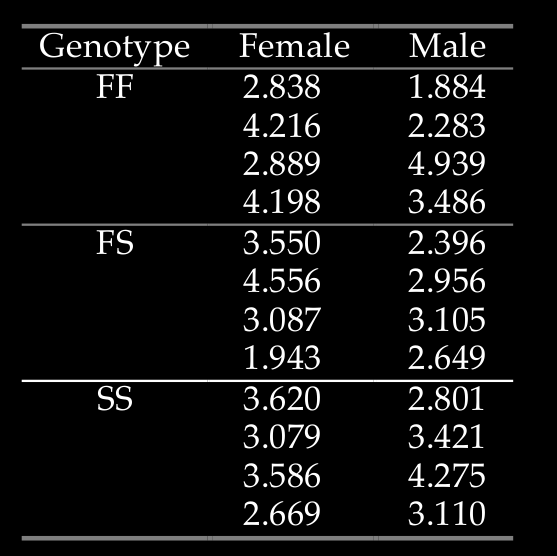
\includegraphics[scale=0.25]{Two-Way-Anova-Data1-neg.png}
				\vfill
				Test at $\alpha=0.05$\\
				\[
				H_0: \mu_F = \mu_M \quad v.s.\quad
				H_1: \mu_F\ne \mu_F
				\]
				and
				\[
					\widetilde H_0: \mu_{FF} = \mu_{S}= \mu_{SS} \quad v.s. \quad \widetilde H_1: \text{not all equal}
				\]
			\end{center}
	\end{enumerate}
\end{frame}
%-------------- end slide -------------------------------%}}}
%-------------- start slide -------------------------------%{{{
\begin{frame}[fragile]
	\begin{minipage}{0.45\textwidth}
	\begin{lstlisting}
> Data
   id    Sex Genotype Activity
1   1   male       ff    1.884
2   2   male       ff    2.283
3   3   male       fs    2.396
4   4 female       ff    2.838
5   5   male       fs    2.956
6   6 female       ff    4.216
7   7 female       ss    3.620
8   8 female       ff    2.889
9   9 female       fs    3.550
10 10   male       fs    3.105
11 11 female       fs    4.556
12 12 female       fs    3.087
13 13   male       ff    4.939
14 14   male       ff    3.486
15 15 female       ss    3.079
16 16   male       fs    2.649
	\end{lstlisting}
	\end{minipage}
	\hfill
	\begin{minipage}{0.45\textwidth}
	\begin{lstlisting}
17 17 female       fs    1.943
18 19 female       ff    4.198
19 20 female       ff    2.473
20 22 female       ff    2.033
21 24 female       fs    2.200
22 25 female       fs    2.157
23 26   male       ss    2.801
24 28   male       ss    3.421
25 29 female       ff    1.811
26 30 female       fs    4.281
27 32 female       fs    4.772
28 34 female       ss    3.586
29 36 female       ff    3.944
30 38 female       ss    2.669
31 39 female       ss    3.050
32 41   male       ss    4.275
33 43 female       ss    2.963
34 46 female       ss    3.236
35 48 female       ss    3.673
36 49   male       ss    3.110
	\end{lstlisting}
	\end{minipage}
\end{frame}
%-------------- end slide -------------------------------%}}}
%-------------- start slide -------------------------------%{{{
\begin{frame}[fragile]
	\begin{minipage}{0.46\textwidth}
	\begin{lstlisting}
> # Two-way ANOVA
> model = lm(Activity ~ Sex + Genotype,
+            data=Data)
> Anova(model, type="II")
Anova Table (Type II tests)

Response: Activity
           Sum Sq Df F value Pr(>F)
Sex        0.0681  1  0.0888 0.7676
Genotype   0.2772  2  0.1808 0.8354
Residuals 24.5285 32
> # One-way ANOVA
> model_Sex = lm(Activity ~ Sex,
+                data=Data)
> Anova(model_Sex, type="II")
Anova Table (Type II tests)

Response: Activity
           Sum Sq Df F value Pr(>F)
Sex        0.0681  1  0.0933 0.7619
Residuals 24.8057 34
> # One-way ANOVA
> model_Genotype = lm(Activity ~ Genotype,
+                data=Data)
> Anova(model_Genotype, type="II")
Anova Table (Type II tests)

Response: Activity
           Sum Sq Df F value Pr(>F)
Genotype   0.2772  2   0.186 0.8312
Residuals 24.5965 33
	\end{lstlisting}
	\end{minipage}
\end{frame}
%-------------- end slide -------------------------------%}}}
%-------------- start slide -------------------------------%{{{
\begin{frame}[fragile]{Tuckey's pairwise comparison}

	\[
		\text{Replace} \quad Q_{\alpha, k,b(k-k)} \quad \text{by}\quad
		Q_{\alpha, k,(b-1)(k-1)}
	\]
	\vfill
	\begin{minipage}{0.47\textwidth}
	\begin{lstlisting}
> # Tukey's pairwise comparison (One-way)
> model1 = aov(Activity ~ Genotype,
+                       data=Data)
> TukeyHSD(model1, "Genotype", ordered = TRUE)
  Tukey multiple comparisons of means
    95% family-wise confidence level
    factor levels have been ordered

Fit: aov(formula = Activity ~ Genotype, data = Data)

$Genotype
            diff        lwr      upr     p adj
fs-ff 0.05483333 -0.8100204 0.919687 0.9867505
ss-ff 0.20741667 -0.6574370 1.072270 0.8272105
ss-fs 0.15258333 -0.7122704 1.017437 0.9021607
	\end{lstlisting}
	\end{minipage}
	\hfill
	\begin{minipage}{0.47\textwidth}
	\begin{lstlisting}
> # Tukey's pairwise comparison (Two-way)
> model2 = aov(Activity ~ Sex + Genotype,
+            data=Data)
> TukeyHSD(model2, "Genotype", ordered = TRUE)
  Tukey multiple comparisons of means
    95% family-wise confidence level
    factor levels have been ordered

Fit: aov(formula = Activity ~ Sex + Genotype, data = Data)

$Genotype
            diff        lwr       upr    p adj
fs-ff 0.05483333 -0.8234920 0.9331586 0.987114
ss-ff 0.20741667 -0.6709086 1.0857420 0.831554
ss-fs 0.15258333 -0.7257420 1.0309086 0.904729
	\end{lstlisting}
	\end{minipage}
\end{frame}
%-------------- end slide -------------------------------%}}}
%-------------- start slide -------------------------------%{{{
\begin{frame}[fragile]

	\begin{enumerate}
		\item[Remark] By two-way ANOVA, or through blocking one factor, we obtain
			\vfill
		\item larger $p$-values:
		\item[] more conservative to reject $H_0$.
			\vfill
		\item wider C.I.'s:
		\item[] more conservative on our estimates.
	\end{enumerate}
\end{frame}
%-------------- end slide -------------------------------%}}}

% \mySection{12.3 Multiple Comparisons: Turkey's Method}
%-------------- start slide -------------------------------%{{{ 12.51
\begin{frame}
	% {\S\: 12.3 Multiple Comparisons: Turkey's Method}
\begin{center}
	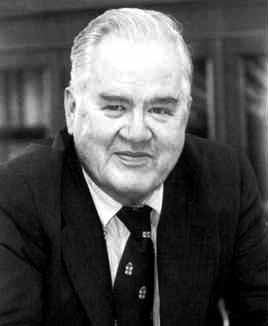
\includegraphics[scale=0.25]{John_Tukey.jpg} \\[2em]
	\small
	\begin{enumerate}
	\item John Wilder Tukey (June 16, 1915 -- July 26, 2000)
		was an American mathematician best known for
		development of the Fast Fourier Transform (FFT) algorithm and box plot.
	\item The Tukey range test, the Tukey lambda distribution,
		the Tukey test of additivity,
		and the Teichm\"uller-Tukey lemma all bear his name.
	\item  He is also credited with coining the term 'bit'.
	\end{enumerate}
	\vfill
	\url{https://en.wikipedia.org/wiki/John_Tukey}
	\end{center}
\end{frame}
%-------------- end slide -------------------------------%}}}
%-------------- start slide -------------------------------%{{{ 12.52
\begin{frame}[fragile]

	\begin{enumerate}
		\item[]
	\begin{center}
		\begin{tabular}{cccc}
			$N(\mu_1,\sigma^2)$ & $N(\mu_2,\sigma^2)$ & $\cdots$ & $N(\mu_2,\sigma^2)$ \\
			\hline
			$Y_{11}$ & $Y_{12}$ & $\cdots$ & $Y_{1k}$\cr
			$Y_{21}$ & $Y_{22}$ & $\cdots$ & $Y_{2k}$\cr
			$\vdots$ & $\vdots$ & $\vdots$ & $\vdots$\cr
			$Y_{r1}$ & $Y_{r2}$ & $\cdots$ & $Y_{rk}$\cr
			\hline
		\end{tabular}
	\end{center}
	\vfill
\item[Goal] For any $i\ne j$, test
	\[
	H_0: \mu_i =\mu_j \qquad v.s. \qquad H_1: \mu_i\ne \mu_j
	\]
	\vfill
\item[] at the $\alpha$ level of significance defined as
	\[
		\bbP \left(\bigcup_{j=1}^{{k\choose 2}}E_j\right) = \alpha
	\]
\item[] where there are ${k\choose 2}$ pairs, and $E_j$ is the event of making a type I error for the $j$-th pair.
	\end{enumerate}

\end{frame}
%-------------- end slide -------------------------------%}}}
%-------------- start slide -------------------------------%{{{ 12.53
\begin{frame}[fragile]
\begin{enumerate}
	\item[Goal'] Simultaneous C.I.'s for ${k\choose 2}$ pairs of means:
	\item[] Given $\alpha$, find $I_{ij}$, the C.I. for $\mu_i-\mu_j$ (with $i,j=1,\cdots,k$ and $i\ne j$), s.t.
	\item[]
		\[
			\bbP\left(\mu_i-\mu_j\in I_{ij},\: \forall i,j=1,\cdots, k, i\ne j\right) = 1-\alpha.
		\]
\end{enumerate}

\end{frame}
%-------------- end slide -------------------------------%}}}
%-------------- start slide -------------------------------%{{{ 12.54
\begin{frame}[fragile]

	\begin{enumerate}
		\item[???] Why not the standard pair-wise two-sample t-test?
		\item[] Suppose $\bbP(E_j)=\alpha_*$. Then
			\begin{align*}
\alpha & = \bbP \left(\bigcup_{j=1}^{{k\choose 2}}E_j\right)
= 1-  \bbP \left(\bigcap_{j=1}^{{k\choose 2}}E_j^c \right)
\approx 1- \prod_{j=1}^{k\choose 2} \bbP(E_j^c)
= 1-(1-\alpha_*)^{k\choose 2}
			\end{align*}
		\item[] Hence,
		\[
			\alpha_* \approx  1-(1-\alpha)^{1/{k\choose 2}}
		\]
		\vfill
	\item[] E.g., $\alpha=0.05$
		\begin{center}
			\begin{tabular}{c|ccc}
				$k$ & 5 & 8 & 100 \\
				\hline
				$\alpha_*$ & 0.0051162 & 0.001830 & 0.00001036
			\end{tabular}
		\end{center}
	\end{enumerate}
\end{frame}
%-------------- end slide -------------------------------%}}}
%-------------- start slide -------------------------------%{{{ 12.55
\begin{frame}[fragile]{Bonferroni's method \\
		\small --- A straightforward method}
		\begin{minipage}{0.4\textwidth}
	\begin{enumerate}
		\item[]
			\begin{align*}
				\bbP\left(\mu_i-\mu_j\in I_{ij},\: \forall i\ne j\right)
			\end{align*}
		\item[]
			\[||\]
			\[
			\bbP\left(\bigcap_{i\ne j}\mu_i-\mu_j\in I_{ij}\right)
			\]
		\item[]
			\[||\]
			\[
				1-\bbP\left(\bigcup_{i\ne j}\mu_i-\mu_j\not\in I_{ij}\right)
			\]
		\item[]
			\[\text{\rotatebox[origin=c]{90}{$\le$}}\]
			\[
				1-\sum_{i\ne j} \bbP\left(\mu_i-\mu_j\not\in I_{ij}\right)
			\]
		\item[]
			\[||\]
			\[
				1 - {k\choose 2} \alpha_*
			\]
	\end{enumerate}
		\end{minipage}
		\hfill\pause
		\begin{minipage}{0.55\textwidth}
			\begin{enumerate}
				\item
			 If we choose $\alpha_* = \alpha/{k\choose 2}$,
		 \item let $I_{ij}$ be the $(1-\alpha_*)100\%$ C.I. $i\ne j$
		 \item[]
			 \[\Downarrow\]
			\begin{align*}
				\bbP\left(\mu_i-\mu_j\in I_{ij},\: \forall i\ne j\right)
			\end{align*}
			\[\text{\rotatebox[origin=c]{90}{$\le$}}\]
			\[
				1 - {k\choose 2} \alpha_*
			\]
			\[||\]
			\[
			1-\alpha.
			\]
			\end{enumerate}
		\end{minipage}
\end{frame}
%-------------- end slide -------------------------------%}}}
%-------------- start slide -------------------------------%{{{ 12.56
\begin{frame}[fragile]

	\begin{enumerate}
\item[Remark] This is an approximation. The resulting C.I. are in general too wide.\\[1em]
\item[] The exact, and much more precise, solution is given by J.W. Turkey.\\[1em]
\item[] One can also construct simultaneous C.I. for all possible linear combinations of the parameters $\sum_{j=1}^k c_j \mu_j$, this can be acchieved by {\bf Scheff\'e's method}. A simple verson is given in \S 12.4.
	\end{enumerate}
\end{frame}
%-------------- end slide -------------------------------%}}}
%-------------- start slide -------------------------------%{{{ 12.57
\begin{frame}[fragile]{Tukey's HSD (honestly significant difference) test}
	\begin{enumerate}
		\item[] Let's construct $(1-\alpha)100\%$ C.I.'s simultaneously for all pairs.
			\vfill
		\item[]
			\[
				\bbP\left(\left|(\overline{Y}_{\cdot i}-\mu_i) - (\overline{Y}_{\cdot j}-\mu_j)\right|\le \mathcal{E},\quad \forall i\ne j\right) = 1-\alpha
			\]
		\item[]
			\[
				||
			\]
			\[
				\bbP\left(\max_{i}(\overline{Y}_{\cdot i}-\mu_i) - \min_{j}(\overline{Y}_{\cdot j}-\mu_j)\le \mathcal{E}\right)\hspace{3em}
			\]
		\item[]
			\[
				||
			\]
			\[
				\bbP\left(\max_{i}\overline{Y}_{\cdot i} - \min_{j}\overline{Y}_{\cdot j}\le \mathcal{E}\right)\hspace{3em}
			\]
			\vfill
		\item[$\Longrightarrow$]  Needs to study  ...
	\end{enumerate}
\end{frame}
%-------------- end slide -------------------------------%}}}
%-------------- start slide -------------------------------%{{{ 12.58
\begin{frame}[fragile]

	\begin{enumerate}
		\item[Def.] Let $W_1,\cdots, W_k$ be $k$ i.i.d. r.v.'s from $N(\mu,\sigma^2)$. Let $R$ denote their range:
		\[
		R =\max_i W_ i -\min_i W_i.
		\]
		Let $S^2$ be an unbiased estimator for $\sigma^2$ independent of the $W_i$'s and based on $\nu$ df.
		Define the {\bf Studentized range, $Q_{k,\nu}$}, to be the ratio:
		\[
			Q_{k,\nu} :=\frac RS.
		\]
		\vfill
	\item[]
		\begin{center}
			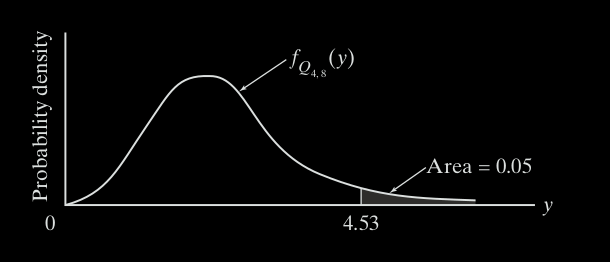
\includegraphics[scale=0.35]{Figure_12-3-1-neg.png}
		\end{center}
	\item[Remark]
		\begin{enumerate}
			\item We need $R\perp S$ to mimic Student's t-distribution.
			\item In the following $\nu = n-k = rk -k = r(k-1)$.
		\end{enumerate}
\end{enumerate}
\end{frame}
%-------------- end slide -------------------------------%}}}
%-------------- start slide -------------------------------%{{{ 12.59
\begin{frame}[fragile]
	\begin{center}

		\begin{enumerate}
			\item[] $Q_{k,\nu}\sim$ {\bf Studentized range distribution} with parameters $k$ and $\nu$.
			\item[] $k$: number of groups.
			\item[] $\nu$: degrees of freedom.
				\vfill
			\item[]
		\end{enumerate}
		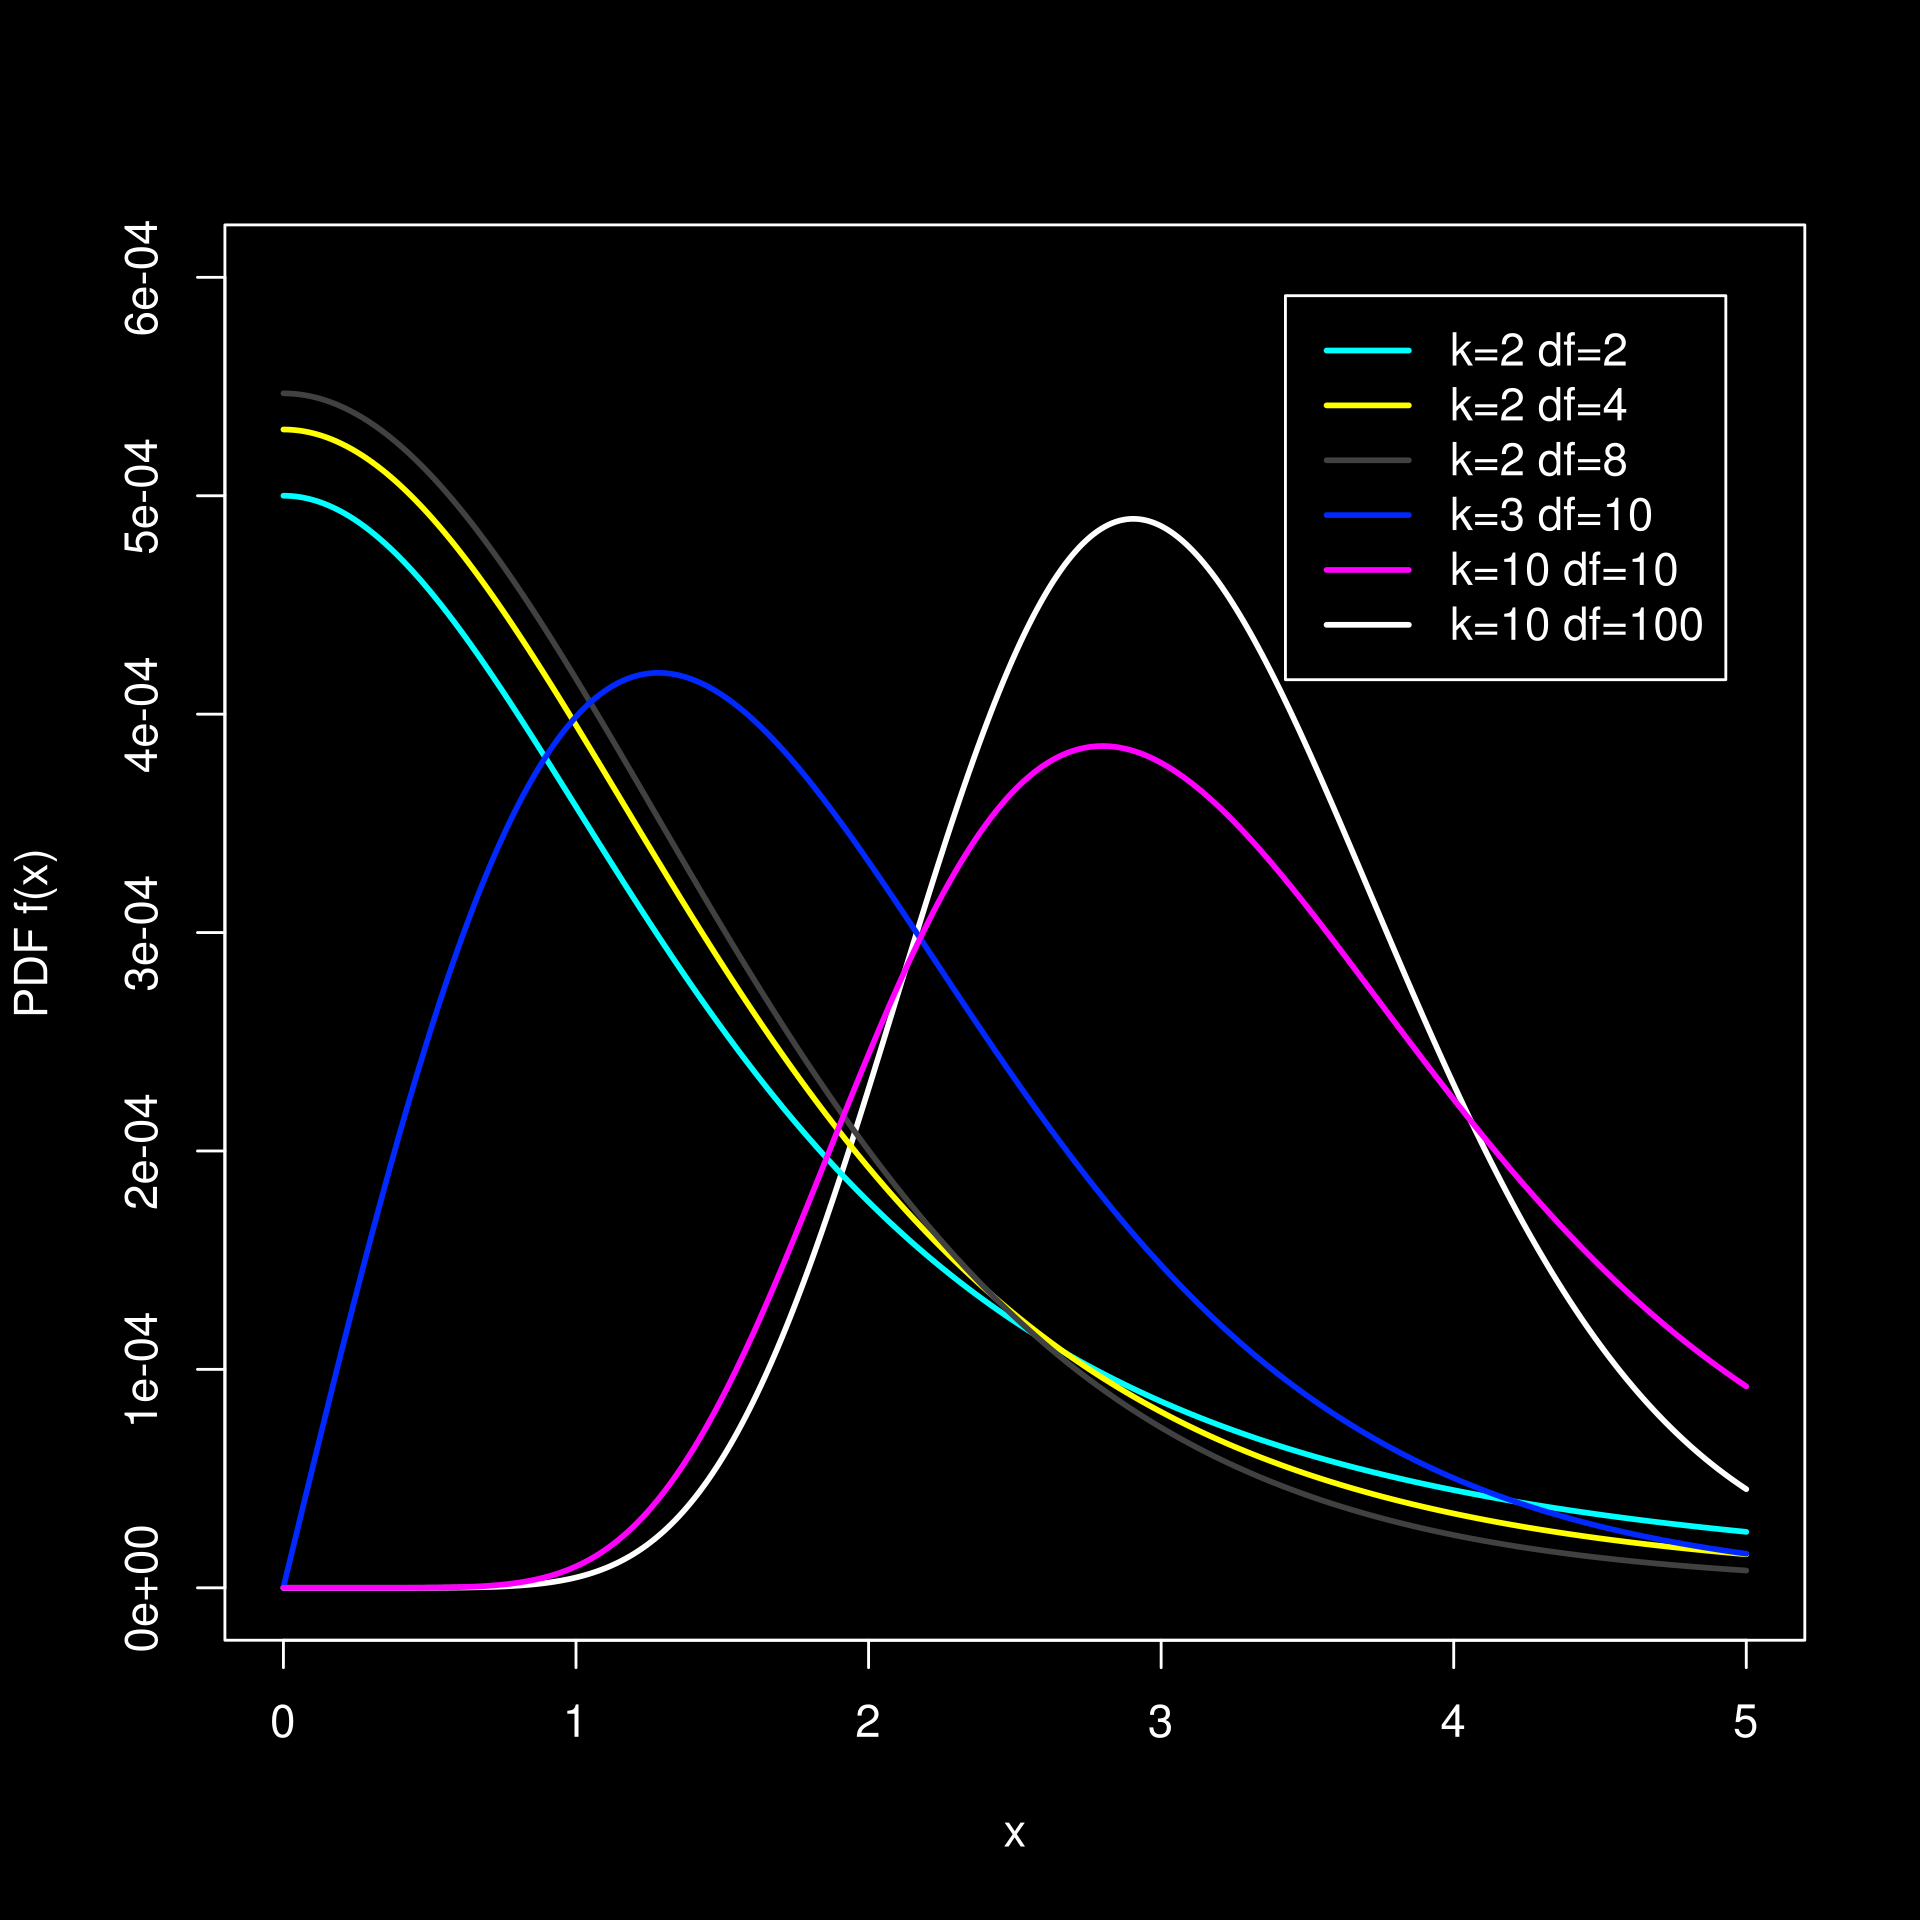
\includegraphics[scale=0.1]{1920px-StudentizedRangePDF.svg-neg.png}
	\end{center}
\end{frame}
%-------------- end slide -------------------------------%}}}
%-------------- start slide -------------------------------%{{{ 12.60
\begin{frame}[fragile]
	Let's find one example that all requirements of the $Q_{k,\nu}$ are satisfied.
	\vfill
	\begin{enumerate}
		\item Take $W_j = \overline{Y}_{\cdot j}-\mu_j$, $j=1,\cdots,k$ $\quad\Longrightarrow\quad$ $W_j\sim N(0,\sigma^2/r)$.
			\vfill
		\item $MSE$ or the pooled variance $S_p^2$ \hfill $MSE/r$
		\item[] \qquad is an unbiased estimator for $\sigma^2$ \hfill $\sigma^2/r$
		\item[] \qquad is $\perp\{\overline{Y}_{\cdot j}\}_{j=1,\cdots, k}$, hence $\perp\{W_j\}_{j=1,\cdots, k}$
			\vfill
		\item $df$ of $MSE$ is equal to $n-k=kr-k = k(r-1)$.
			\vfill
		\item[$\Longrightarrow$] \hspace{1em} $\displaystyle \frac{\max_{i}W_i - \min_j W_j}{\sqrt{MSE/r}} \sim $ Studentized range distribution($k$, $rk-k$)
	\end{enumerate}
\end{frame}
%-------------- end slide -------------------------------%}}}
%-------------- start slide -------------------------------%{{{ 12.61
\begin{frame}[fragile]

	\begin{enumerate}
		\item[]
	\[
		\hspace{3em}		\bbP \left( \frac{\max_{i}W_i - \min_j W_j}{\sqrt{MSE/r}} \le Q_{\alpha,k,rk-k}  \right ) = 1-\alpha
	\]
		\item[]
	\[||\]
	\[
		\bbP \left(\max_i W_i -\min_j W_j \le \frac{Q_{\alpha,k,rk-k}}{\sqrt{r}}\sqrt{MSE}\right)
	\]
		\item[]
	\[||\]
	\[
		\bbP \left(\left| W_i -W_j\right| \le \frac{Q_{\alpha,k,rk-k}}{\sqrt{r}}\sqrt{MSE},\:\:\forall i\ne j\right)
	\]
		\item[]
	\[||\]
	\[
		\bbP \left(\left| \left(\overline{Y}_{\cdot i} -\overline{Y}_{\cdot j}\right) - (\mu_i-\mu_j)\right| \le \frac{Q_{\alpha,k,rk-k}}{\sqrt{r}}\sqrt{MSE},\:\:\forall i\ne j\right)
	\]
		\item[]
	\[||\]
	\[
		\hspace{-2em}		\bbP \left(
			\overline{Y}_{\cdot i} -\overline{Y}_{\cdot j} - \frac{Q_{\alpha,k,rk-k}}{\sqrt{r}}\sqrt{MSE}
		\le \mu_i-\mu_j \le
			\overline{Y}_{\cdot i} -\overline{Y}_{\cdot j}+ \frac{Q_{\alpha,k,rk-k}}{\sqrt{r}}\sqrt{MSE}
		,\:\: \forall i\ne j\right )
	\]
	\end{enumerate}
\end{frame}
%-------------- end slide -------------------------------%}}}
%-------------- start slide -------------------------------%{{{ 12.62
\begin{frame}[fragile]

	\begin{enumerate}
		\item[] Therefore, for all $i\ne j$,
			the $100(1-\alpha)\%$ C.I. for $ \mu_i-\mu_j $ is \\[2em]
			\[
			\overline{Y}_{\cdot i} -\overline{Y}_{\cdot j} \pm  \frac{Q_{\alpha,k,rk-k}}{\sqrt{2}}\sqrt{MSE}\sqrt{\frac 2r}
			\]
			\vfill
		\item[] To test $H_0: \mu_i=\mu_j$ for specific $i\ne j$, reject $H_0$ in favor of $H_1:\mu_i\ne\mu_j$ if the C.I. does NOT contain $0$, at the $\alpha$ level of significance.\myEnd
			\vfill
		\item[Note:] When sample sizes are not equal, use the {\bf Tukey-Kramer method}: \\[2em]
			\[
				\overline{Y}_{\cdot i} -\overline{Y}_{\cdot j} \pm  \frac{Q_{\alpha,k,rk-k}}{\sqrt{2}}\sqrt{MSE}\sqrt{\frac{1}{r_i} + \frac{1}{r_j}}
			\]
	\end{enumerate}
\end{frame}
%-------------- end slide -------------------------------%}}}
%-------------- start slide -------------------------------%{{{ 12.63
\begin{frame}
	\begin{enumerate}
		\item[E.g. 2] A certain fraction of antibiotics injected into the bloodstream are ``bound'' to
serum proteins. This phenomenon bears directly on the effectiveness of the
medication, because the binding decreases the systemic uptake of the drug.
Table below lists the binding percentages in bovine serum measured for five
widely prescribed antibiotics. Which antibiotics have similar binding
properties, and which are different? \\[1em]
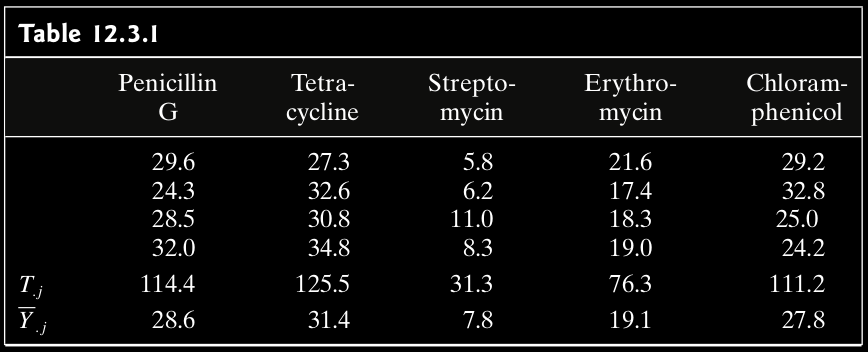
\includegraphics[scale=0.25]{Table_12-3-1-neg.png}
	\end{enumerate}
\end{frame}
%-------------- end slide -------------------------------%}}}
%-------------- start slide -------------------------------%{{{ 12.64
\begin{frame}[fragile]
	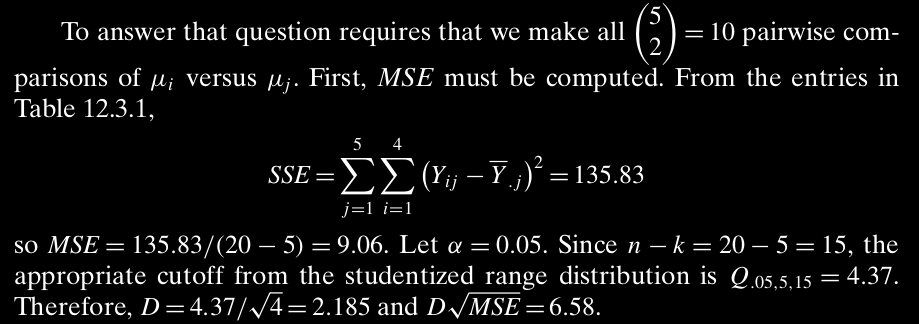
\includegraphics[scale=0.28]{Case_12-3-1-Sol1-neg.png}\\
	\vfill
	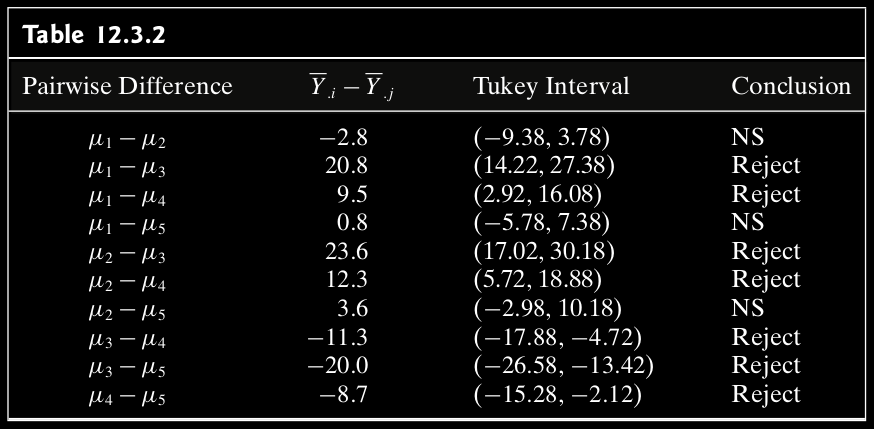
\includegraphics[scale=0.3]{Table_12-3-2-neg.png}
\end{frame}
%-------------- end slide -------------------------------%}}}
%-------------- start slide -------------------------------%{{{ 12.65
\begin{frame}[fragile]
	\begin{minipage}{0.3\textwidth}
	\begin{lstlisting}
> # Case Study 12.3.1
> # Input data first
> Input <- c("
+ rates group
+ 29.6  M1
+ 24.3  M1
+ 28.5  M1
+ 32.0  M1
+ 27.3  M2
+ 32.6  M2
+ 30.8  M2
+ 34.8  M2
+ 5.8   M3
+ 6.2   M3
+ 11.0  M3
+ 8.3   M3
+ 21.6  M4
+ 17.4  M4
+ 18.3  M4
+ 19.0  M4
+ 29.2  M5
+ 32.8  M5
+ 25.0  M5
+ 24.2 M5
+ ")
> Data = read.table(
 	textConnection(Input),
+       header=TRUE)
	\end{lstlisting}
	\end{minipage}
	\begin{minipage}{0.63\textwidth}
	\begin{lstlisting}
> # Compute one-way ANOVA test
> res.aov <- aov(rates ~ group, data = Data)
> # Summary of the analysis
> summary(res.aov)
            Df Sum Sq Mean Sq F value   Pr(>F)
group        4 1480.8   370.2   40.88 6.74e-08 ***
Residuals   15  135.8     9.1
---
Signif. codes:  0 '***' 0.001 '**' 0.01 '*' 0.05 '.' 0.1 ' ' 1
	\end{lstlisting}
	\end{minipage}

\end{frame}
%-------------- end slide -------------------------------%}}}
%-------------- start slide -------------------------------%{{{ 12.66
\begin{frame}[fragile]
	\begin{center}
		\begin{minipage}{0.6\textwidth}
	\begin{lstlisting}
> # Tukey multiple pairwise-comparisons
> TukeyHSD(res.aov)
  Tukey multiple comparisons of means
    95% family-wise confidence level

Fit: aov(formula = rates ~ group, data = Data)

$group
         diff        lwr        upr     p adj
M2-M1   2.775  -3.795401   9.345401 0.6928357
M3-M1 -20.775 -27.345401 -14.204599 0.0000006
M4-M1  -9.525 -16.095401  -2.954599 0.0034588
M5-M1  -0.800  -7.370401   5.770401 0.9952758
M3-M2 -23.550 -30.120401 -16.979599 0.0000001
M4-M2 -12.300 -18.870401  -5.729599 0.0003007
M5-M2  -3.575 -10.145401   2.995401 0.4737713
M4-M3  11.250   4.679599  17.820401 0.0007429
M5-M3  19.975  13.404599  26.545401 0.0000010
M5-M4   8.725   2.154599  15.295401 0.0071611
	\end{lstlisting}
		\end{minipage}
	\end{center}
\end{frame}
%-------------- end slide -------------------------------%}}}
%-------------- start slide -------------------------------%{{{ 12.67
\begin{frame}[fragile]
	\begin{center}
		\begin{minipage}{0.6\textwidth}
	\begin{lstlisting}
> round(TukeyHSD(res.aov)$group,2)
					diff   		 lwr		    upr		 p adj
M2-M1		   2.78		  -3.80		   9.35		  0.69
M3-M1		 -20.77		 -27.35		 -14.20		  0.00
M4-M1		  -9.52		 -16.10		  -2.95		  0.00
M5-M1		  -0.80		  -7.37		   5.77		  1.00
M3-M2		 -23.55		 -30.12		 -16.98		  0.00
M4-M2		 -12.30		 -18.87		  -5.73		  0.00
M5-M2		  -3.58		 -10.15		   3.00		  0.47
M4-M3		  11.25		   4.68		  17.82		  0.00
M5-M3		  19.97		  13.40		  26.55		  0.00
M5-M4		   8.73		   2.15		  15.30		  0.01
---
Signif. codes:  0 '***' 0.001 '**' 0.01 '*' 0.05 '.' 0.1 ' ' 1
(Adjusted p values reported -- single-step method)
	\end{lstlisting}
		\end{minipage}
		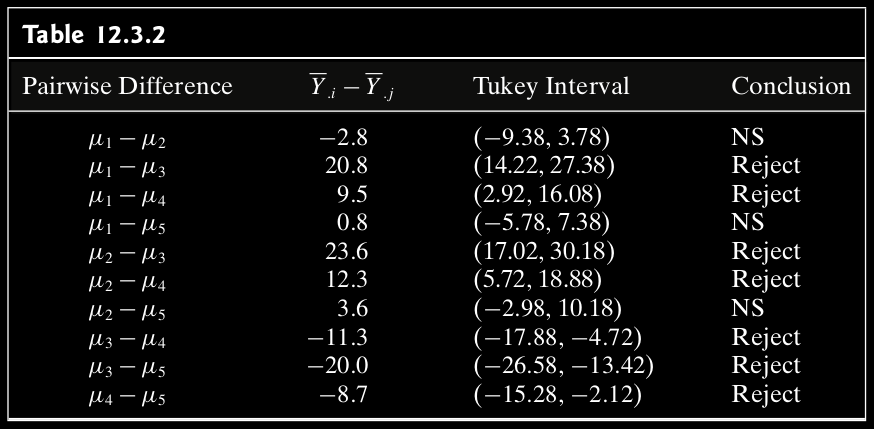
\includegraphics[scale=0.25]{Table_12-3-2-neg.png}
	\end{center}
\end{frame}
%-------------- end slide -------------------------------%}}}
%-------------- start slide -------------------------------%{{{ 12.68
\begin{frame}[fragile]
	\begin{center}
		\begin{minipage}{0.7\textwidth}
	\begin{lstlisting}
	> # Or one may use multcomp package or multiple comparisons
> library(multcomp)
> summary(glht(res.aov, linfct = mcp(group = "Tukey")))

	 Simultaneous Tests for General Linear Hypotheses

Multiple Comparisons of Means: Tukey Contrasts


Fit: aov(formula = rates ~ group, data = Data)

Linear Hypotheses:
             Estimate Std. Error t value Pr(>|t|)
M2 - M1 == 0    2.775      2.128   1.304  0.69283
M3 - M1 == 0  -20.775      2.128  -9.764  < 0.001 ***
M4 - M1 == 0   -9.525      2.128  -4.477  0.00348 **
M5 - M1 == 0   -0.800      2.128  -0.376  0.99528
M3 - M2 == 0  -23.550      2.128 -11.068  < 0.001 ***
M4 - M2 == 0  -12.300      2.128  -5.781  < 0.001 ***
M5 - M2 == 0   -3.575      2.128  -1.680  0.47374
M4 - M3 == 0   11.250      2.128   5.287  < 0.001 ***
M5 - M3 == 0   19.975      2.128   9.388  < 0.001 ***
M5 - M4 == 0    8.725      2.128   4.101  0.00717 **
---
Signif. codes:  0 '***' 0.001 '**' 0.01 '*' 0.05 '.' 0.1 ' ' 1
(Adjusted p values reported -- single-step method)
	\end{lstlisting}
		\end{minipage}
	\end{center}
\end{frame}
%-------------- end slide -------------------------------%}}}
%-------------- start slide -------------------------------%{{{ 12.69
\begin{frame}[fragile]
	\begin{center}
		\begin{minipage}{0.7\textwidth}
	\begin{lstlisting}
	             Estimate Std. Error t value Pr(>|t|)
M2 - M1 == 0    2.775      2.128   1.304  0.69283
M3 - M1 == 0  -20.775      2.128  -9.764  < 0.001 ***
M4 - M1 == 0   -9.525      2.128  -4.477  0.00348 **
M5 - M1 == 0   -0.800      2.128  -0.376  0.99527
M3 - M2 == 0  -23.550      2.128 -11.068  < 0.001 ***
M4 - M2 == 0  -12.300      2.128  -5.781  < 0.001 ***
M5 - M2 == 0   -3.575      2.128  -1.680  0.47371
M4 - M3 == 0   11.250      2.128   5.287  < 0.001 ***
M5 - M3 == 0   19.975      2.128   9.388  < 0.001 ***
M5 - M4 == 0    8.725      2.128   4.101  0.00719 **
	\end{lstlisting}
		\end{minipage}
		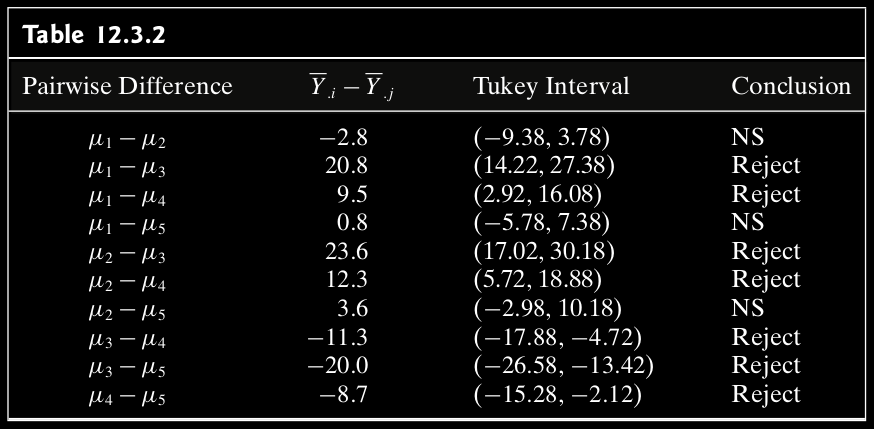
\includegraphics[scale=0.25]{Table_12-3-2-neg.png}
	\end{center}
\end{frame}
%-------------- end slide -------------------------------%}}}
%-------------- start slide -------------------------------%{{{ 12.70
\begin{frame}{Two more examples of ANOVA using R}
	\begin{enumerate}
		\item[E.g. 1] \url{http://www.sthda.com/english/wiki/one-way-anova-test-in-r}
			\vfill
		\item[E.g. 2] \url{https://datascienceplus.com/one-way-anova-in-r/}
	\end{enumerate}
\end{frame}
%-------------- end slide -------------------------------%}}}

% \mySection{12.4 Testing Subhypotheses with Contrasts}
%-------------- start slide -------------------------------%{{{ 12.73
\begin{frame}
		% {\S\: 12.4 Testing Subhypotheses with Contrasts}
\end{frame}
%-------------- end slide -------------------------------%}}}

\end{document}

